\documentclass[11pt,a4paper]{article}
\usepackage[utf8]{inputenc}
\usepackage[english]{babel}
\usepackage[T1]{fontenc}
\usepackage{charter}
\usepackage{amsmath}
\usepackage{amsfonts}
\usepackage{amssymb}
\usepackage{esint}
\usepackage[table]{xcolor}
\usepackage{graphicx}
\usepackage[left=1.5cm,right=1.5cm,top=2cm,bottom=2cm]{geometry}
\usepackage{tikz}
\usepackage{tikz-3dplot}
\usetikzlibrary{babel}
\usetikzlibrary{calc,patterns,decorations.pathmorphing,decorations.markings}
\usepackage[font=small,labelfont={small,bf},margin=0.5cm,justification=justified]{caption}
\usepackage[font=small,labelfont={small,bf}]{subcaption}
\usepackage{epstopdf}
\usepackage{natbib}
\usepackage[nointegrals]{wasysym}
%\renewcommand\familydefault\sfdefault
\usepackage[italic,defaultmathsizes]{mathastext}
\usepackage{hyperref}
\usepackage{lipsum}
\usepackage{threeparttable}
\usepackage{titling}
\usepackage[bf]{titlesec}
\usepackage{abstract}
\usepackage{lastpage}
\usepackage{fancyhdr}
\usepackage{csvsimple}
\usepackage{longtable}
\usepackage{pdflscape}
\usepackage{authblk}
\usepackage{calculator}
\usepackage{multirow}

\hypersetup{
%      draft,
   linktocpage=true,
    colorlinks=true,
    linkcolor=blue,
    citecolor=blue,
    filecolor=blue,      
    urlcolor=blue
}

\tikzset{>=latex}
\usetikzlibrary{arrows}
\pgfarrowsdeclarecombine{latexo}{latexo}
{*}{latex}{latex}{*}

%\numberwithin{equation}{section}
\renewcommand\Authfont{\large}
\renewcommand\Affilfont{\small}
%\renewcommand\abstractnamefont{\fontfamily{qcr}\selectfont}

\pretitle{\begin{center}\LARGE\bfseries}
\posttitle{\end{center}}

\titlelabel{\thetitle. \,}

\author[1,2]{Santiago H. Luna}

\affil[1]{Instituto de Estudios Andinos ``Don Pablo Groeber'' (\textsc{idean}). Universidad De Buenos Aires -- \textsc{conicet}.}
\affil[2]{Instituto de Tecnología e Ingeniería. Universidad Nacional de Hurlingham.}

\title{thermev2 -- A thermal model for the Earth} 

\date{\today}

\pagestyle{fancy}

\fancypagestyle{firststyle}
{
      \fancyhf{}
      \chead{\small{Manuscript -- File name: \textit{thermev2 doc} -- Version 1}}
      \lfoot{Corresponding author: Santiago Luna (\href{mailto:sluna@gl.fcen.uba.ar}{sluna@gl.fcen.uba.ar})}
      \rfoot{Page \thepage \ of \pageref{LastPage}}
      \renewcommand{\headrulewidth}{0.4pt}
      \renewcommand{\footrulewidth}{0.4pt}
}

\fancyhf{}
\lhead{\small{thermev2 -- A thermal model for the Earth}}
\rhead{\small{Luna, S.H.}}
\cfoot{Page \thepage \ of \pageref{LastPage}}
\renewcommand{\headrulewidth}{0.4pt}
\renewcommand{\footrulewidth}{0.4pt}

\newcommand{\sgn}{\mathop{\text{sgn}}}
\newcommand{\apj}{The Astrophysical Journal}
\newcommand{\diff}[0]{\text{d}}
\newcommand{\fdiff}[2]{\frac{\text{d} #1}{\text{d} #2}}
\newcommand{\pdiff}[2]{\frac{\partial #1}{\partial #2}}
\newcommand{\fddiff}[2]{\frac{\text{d^2} #1}{\text{d} #2^2}}
\newcommand{\degr}[0]{^{\circ}}
\newcommand{\chel}[4]{^{#1}_{#2}\text{#3}^{#4}}
\newcommand{\valmed}[1]{\left\langle #1 \right\rangle}
\newcommand{\E}[1]{\times 10^{#1}}
\renewcommand{\vec}[1]{\mathbf{#1}}
\newcommand{\vecg}[1]{\boldsymbol{#1}}
\newcommand{\iu}{\text{i}}
\newcommand{\norm}[1]{\left\vert\left\vert #1 \right\vert\right\vert}
\newcommand{\abs}[1]{\left\vert #1 \right\vert}
\renewcommand{\arraystretch}{1.5}
\newcommand{\apendice}{
      \appendix\numberwithin{equation}{section}
      \titleformat{\section}{\Large\bfseries}{\appendixname \ \thesection .}{0.35em}{}
      \titleformat{\subsection}{\large\bfseries}{\thesubsection .}{0.35em}{}
      \titleformat{\subsubsection}{\normalsize\bfseries}{\thesubsubsection .}{0.35em}{}
}

\tdplotsetmaincoords{70}{110}

\begin{document}

\maketitle

\thispagestyle{firststyle}

\section{Introduction\label{sec:intro}}

This document provides a description of a model to simulate the thermal evolution of the Earth's interior, that is, the time evolution of the characteristic temperatures of the mantle and core of the Earth throughout its history, which is mainly based on the models developed by \citet{stevensonetal1983} and \citep{tosietal2017} including the heat generated by tidal interaction.

The earth is considered to be divided into two parts: the core and the mantle (see Fig.~\ref{fig:Earth_interior}). Both are bounded by two concentric spherical surfaces, an outer one of radius $R_\oplus$, which is the mean radius of the Earth, and the inner one of radius $R_\text{c}$, which is equal to the radius of the core. The latter defines the core-mantle boundary (CMB).

\begin{figure*}[t]
      \centering
      \begin{subfigure}[b]{0.45\textwidth}
      \centering
      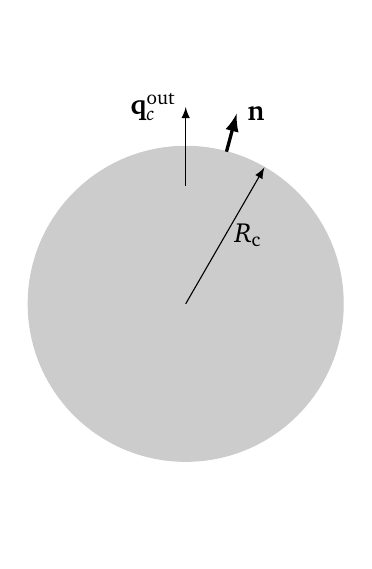
\begin{tikzpicture}
      \draw[dashed,white] (0,-3) -- (0,3.5);
      \filldraw[black!20!white] (0,0) circle [radius=2cm];
      \draw[->] (0,0) -- node[midway,right]{$R_{\text{c}}$}(60:2cm);
      \draw[->] (90:1.5cm) -- (90:2.5cm) node[left]{$\mathbf{q}^{\text{out}}_c$};
      \draw[very thick,->] (75:2cm) -- (75:2.5cm) node[right]{$\mathbf{n}$};
      \end{tikzpicture}
      \caption{Heat flow through core's surface.}
      \label{fig:flujo_nucleo}
      \end{subfigure}
~
      \begin{subfigure}[b]{0.45\textwidth}
       \centering
       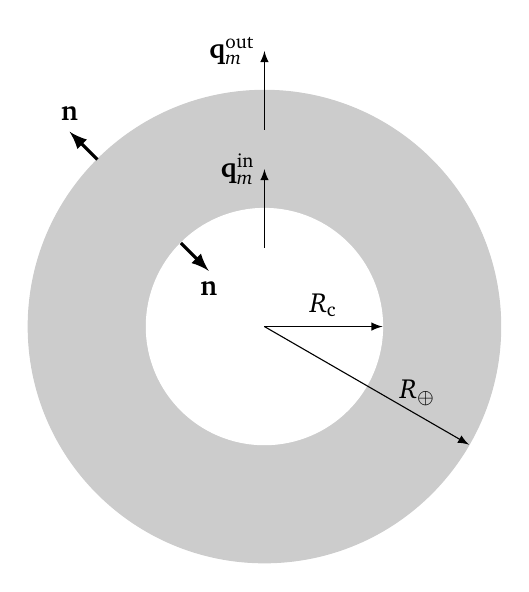
\begin{tikzpicture}
       \draw[dashed,white] (0,-3) -- (0,3.5);
       \filldraw[black!20!white] (0,0) circle [radius=3cm];
       \filldraw[white] (0,0) circle [radius=1.5cm];
       \draw[->] (0,0) -- node[midway,above]{$R_{\text{c}}$}(0:1.5cm);
       \draw[->] (0,0) --  node[near end,above]{$R_{\oplus}$}(-30:3cm);
       \draw[->] (90:1cm) -- (90:2cm) node[left]{$\mathbf{q}^{\text{in}}_m$};
       \draw[->] (90:2.5cm) -- (90:3.5cm) node[left]{$\mathbf{q}^{\text{out}}_m$};
       \draw[very thick,->] (135:3cm) -- (135:3.5cm) node[above]{$\mathbf{n}$};
       \draw[very thick,<-] (135:1cm)node[below]{$\mathbf{n}$} -- (135:1.5cm);
      \end{tikzpicture}
      \caption{Heat flow through inner and outer surfaces of the mantle.}
      \label{fig:flujo_manto}
      \end{subfigure}
      \caption{\label{fig:Earth_interior} Schematics of the Earth's interior structure. Heat flow through the core surface (\subref{fig:flujo_nucleo}) and the inner and outer surfaces of the mantle (\subref{fig:flujo_manto}).}
\end{figure*}

Both the thermal evolution of the core and the mantle are obtained from the energy balance within each layer. Thus, the time evolution of the average internal temperatures of the mantle and core are determined by the balance between the incoming and outgoing heat flux, heat sources and sinks. Among the energy sources are considered radiative decay, both in the mantle and in the core, and the aforementioned tidal interaction, which is assumed to be uniformly distributed in the mantle only. The energy sinks of the mantle are the heat that propagates by convection from the core to the surface and the heat absorbed or released upon melting or solidification of the material that composes the mantle.

\section{Theoretical background\label{sec:theory}}

Let us begin from first principles. Both, the core and mantle, are considered as two separated systems in contact. The thermal states of each of them is characterized by their internal energy, $U$. Since temperatures within Earth's core and mantle are considered to vary with time, then their internal energies will also be time-dependant. The time evolution of $U$ can be tracked by the continuity equation:
\begin{equation}
      \label{ec:Ucontinuity}
      \fdiff{U}{t} + \oiint_S \vec{q} \cdot \text{d} \vec{S} = \fdiff{U_\text{gen}}{t},
\end{equation} where $t$ is time, $\vec{q}$ is the energy flux, which is integrated over a closed surface $S$, and the the term on the right hand side of Eq.~\eqref{ec:Ucontinuity} is the time rate at which the internal energy is generated by sources inside the surface. 

Now, let us rewrite Eq.~\eqref{ec:Ucontinuity} in a more convenient form. To this end, we will consider the first principle of thermodynamics, which relates the change of internal energy ($\Delta U$), the amount of heat exchanged ($Q$), and work ($W$) as:
\begin{equation}
      \label{ec:first_pple}
      \Delta U = Q - W.
\end{equation} Work is related to volume change of the considered system. However, we assume that the volume of both the core and the mantle are fixed, then $W = 0$, and:
\begin{equation}
      \label{ec:first_pple_UQ}
      \Delta U = Q,
\end{equation} that is, the internal energy changes because of exchange of heat between core and mantle, and between mantle and external space. Thus, Eq.~\eqref{ec:Ucontinuity} is rewritten as:
\begin{equation}
      \label{ec:Qcontinuity}
      \fdiff{Q}{t} + \oiint_S \vec{q} \cdot \text{d} \vec{S} = \fdiff{Q_\text{gen}}{t},
\end{equation} where $\vec{q}$ can now formally be identified as the heat flux. Let us consider first the expression of the amount of heat exchanged. For both the core and the mantle we will assume that the heat transferred produces a change in the temperatures ($\Delta T$) and partial melting. Thus, $Q$ is given by:
\begin{equation}
      \label{ec:Qgral}
      Q = M \, c \, \Delta T + L \, M_\text{melt},
\end{equation} where $M$ is the mass, $c$ is the specific heat, $L$ is the latent heat, and $M_\text{melt}$ is the mass of molten or solidified material. Like the volume, the masses of the core and mantle are also assumed constant as well as their physical parameter such as the specific and latent heat. Thus, the rate of change of exchanged heat is associated to changes in temperatures and mass of molten materials. Then, we have:
\begin{equation}
      \label{ec:dQdtgral}
      \fdiff{Q}{t} = M \, c \, \fdiff{T}{t} + L \, \fdiff{M_\text{melt}}{t}.
\end{equation} As we will be explained later, temperature varies within both mantle and core and we will assume that their internal temperatures are function of time and depth (or distance from Earth center, $r$). Since Eq.~\eqref{ec:dQdtgral} is valid for the core and mantle each of them considered as a whole, then the symbol $T$ actually stands for the mean temperature of each layer.

Let us consider now the second term on the left hand side of Eq.~\eqref{ec:Qcontinuity}. In order to compute the surface integral, the core and the mantle need to be considered separately. First of all, in both cases the heat is assumed to flow radially from the Earth's center to its surface. Thus, the heat flux can be expressed as $\vec{q} (t) = q (t) \, \hat{\vec{r}}$, where $\hat{\vec{r}}$ is a unit vector pointing outwards the Earth in radial direction. In addition, the surface element $\text{d} \vec{S}$ can be rewritten as $\text{d} \vec{S} = \vec{n} \, \text{d}S$, where $\vec{n}$ is an unit vector normal to each limiting surface. So, in general, we have that $\vec{q} (t) \cdot \text{d} \, \vec{S} = q (t) \, \text{d}S \left(\hat{\vec{r}} \cdot \vec{n}\right) = \pm q (t) \, \text{d}S$, depending on whether unit vectors $\vec{n}$ and $\hat{\vec{r}}$ have the same or opposite direction. For the core we have that $\vec{q}_c^\text{out} (t) \cdot \text{d} \, \vec{S} = q_c^\text{out} (t) \, \text{d}S$, because unit vectors $\vec{n}$ and $\hat{\vec{r}}$ have the same direction, as can be noted from Fig.~\ref{fig:flujo_nucleo}. In consequence:
\begin{equation}
      \label{ec:oint_core}
      \oiint_{S_c} \vec{q}_c^\text{out} \cdot \text{d} \vec{S} = \oiint_{S_c} q_c^\text{out} (t) \, \text{d}S = q_c^\text{out} (t) \oiint_{S_c} \text{d}S = q_c^\text{out} (t) \, A_c
\end{equation} where $S_c$ indicates that the integration is performed over the core's surface and $A_c$ is the surface area of the core. In the case of the mantle, the surface integral must be divided into two parts, one Corresponding to the inner limiting surface and the other to the outer limiting surface:
\begin{equation}
      \label{ec:oint_mantle}
      \begin{split}
            \oiint_{S_m} \vec{q}_m^\text{out} \cdot \text{d} \vec{S} &= \oiint_{S_m^\text{inner}} \vec{q}_m^\text{in} \cdot \text{d} \vec{S} + \oiint_{S_m^\text{outer}} \vec{q}_m^\text{out} \cdot \text{d} \vec{S} \\
            &= \oiint_{S_{m}^\text{inner}} q_m^\text{in} (t) \, \text{d}S
      \end{split}
\end{equation} The computation of the second integral on the right hand side of Eq.~\eqref{ec:oint_mantle} is totally analogous to the case of the core. Thus:
\begin{equation}
      \label{ec:oint_mantle_outer}
      \oiint_{S_m^\text{outer}} \vec{q}_m^\text{out} \cdot \text{d} \vec{S} = \oiint_{S_m^\text{outer}} q_m^\text{out} (t) \, \text{d}S = q_m^\text{out} (t) \, A_\oplus,
\end{equation} where $A_\oplus$ is the surface area of the Earth. As for the first integral on the right hand side of Eq.~\eqref{ec:oint_mantle}, we have to take into account, on one hand, that the dot product is negative because $\hat{\vec{r}}$ and $\vec{n}$ have opposite directions and, on the other hand, that the inner surface area of the mantle is equal to the core's surface area, i.e. $S_{m}^\text{inner} = S_c$. Then:
\begin{equation}
      \label{ec_oint_mantle_inner}
      \oiint_{S_m^\text{inner}} \vec{q}_m^\text{in} \cdot \text{d} \vec{S} = \oiint_{S_m^\text{inner}} q_m^\text{in} (t) \, \text{d}S = q_m^\text{in} (t) \, A_c.
\end{equation} Moreover, for continuity reasons, and because Earth's core and mantle are in contact with each other, we have that $q_m^\text{in} (t) = q_c^\text{out} (t) = q_\textsc{cmb} (t)$.

Lastly, as we pointed out before, we assume that radioactive decay is a heat source for both the core and the mantle, while tidal heating is present only in the latter. Thus, for the core we have that
\begin{equation}
      \label{ec:dQgendt_core}
      \fdiff{Q_\text{gen}}{t} = \dot{Q}_\text{rad,c},
\end{equation} and for the mantle:
\begin{equation}
      \label{ec:mantle}
      \fdiff{Q_\text{gen}}{t} = \dot{Q}_\text{rad,m} + \dot{Q}_\text{tidal}.
\end{equation}

Then, putting everything together we arrive to the equation governing the thermal evolution of both the core and the mantle:
\begin{align}
      M_c \, c_c \, \fdiff{\valmed{T}_c}{t} + \left(L_c + E_G\right) \, \fdiff{M_\text{ic}}{t} + \dot{Q}_\textsc{cmb} (t) &= \dot{Q}_\text{rad,c} (t) \label{ec:dTmdt_core_gral} \\
      M_m \, c_m \, \fdiff{\valmed{T}_m}{t} + L_m \, \fdiff{M_\text{melt}}{t} - \dot{Q}_\textsc{cmb} (t) + \dot{Q}_\text{conv} (t) &= \dot{Q}_\text{rad,m} (t) + \dot{Q}_\text{tidal} (t), \label{ec:dTmdt_mantle_gral}
\end{align} where the subscripts $c$ and $m$ refers to quantities related to the core and mantle, respectively, $\valmed{T}_i$ (with $i=c,m$) denotes the average temperature of each layer, $\dot{Q}_\textsc{cmb} (t) = q_\textsc{cmb} (t) \, A_c$ and $\dot{Q}_\text{conv} = q_m^\text{out} \, A_\oplus$.

The second term on the left hand side of both Eq.~\eqref{ec:dTmdt_core_gral} and Eq.~\eqref{ec:dTmdt_mantle_gral} are slightly different from that of Eq.~\eqref{ec:dQdtgral} because melting or solidification process in the core and the mantle are different from each other. While the mass of molten material in the mantle, denoted by $M_\text{melt}$, is concentrated in a zone called asthenosphere, which is near the Earth's surface, we assume that the core is completely molten at the beginning of the Earth's history and that solidified core materials precipitate to Earth's center as it cools down forming a solid inner core. Thus, the mass of solidified material within the core is equal to the inner core mass ($M_\text{ic}$). In addition we take into account the gravitational energy release upon solidification of core materials through the parameter $E_G$, which is assumed constant.

In the following subsections, the expressions of the heat fluxes, heat sources, and time rates of melt mass in the mantle and of the inner core mass will be given.

\subsection{Temperature profile of the Earth's interior}

On geological timescales, the dominant heat transport mechanism is convection. For the sake of simplicity, we assume a whole mantle convection \citep{stevensonetal1983}. However, models considering two layers convection within mantle has been developed \citep[and references therein]{schubertetal2001}. The vigor of convection can be measured by the Rayleigh number (Ra). In the case of a fluid limited by two horizontal surfaces and heated from below, analog to Earth's conditions, the Rayleigh number is given by:
\begin{equation}
      \label{ec:Rayleigh_num_def}
      \text{Ra} = \frac{\rho \, \alpha \, g \, \Delta T \, L^3}{\kappa \, \eta (T)},
\end{equation} where $\rho$, $\alpha$, $\kappa$ and $\eta$ are the fluid's density, volumetric expansion coefficient, thermal diffusivity, and dynamical viscosity, respectively, while $\Delta T$ is the temperature jump across the layer of thickness $L$. In Eq.~\eqref{ec:Rayleigh_num_def} we have included the strong dependence of the viscosity on the temperature, which is evaluated at a characteristic temperature of the layer. If Rayleigh number is above some threshold, called the critical Rayleigh number ($\text{Ra}_\text{cr}$), then heat is transported by convection and if it is below that threshold, then heat is transferred by conduction.

\begin{figure}
    \centering
    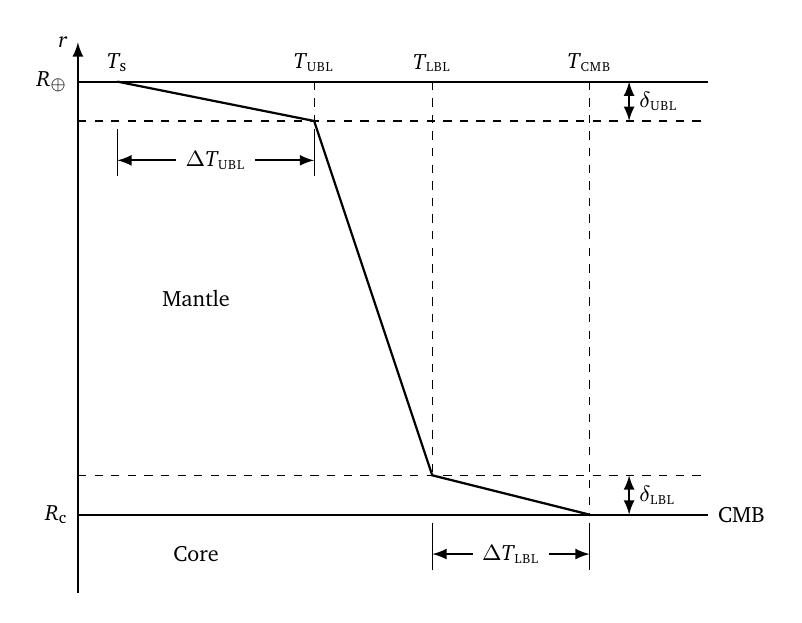
\begin{tikzpicture}[scale=1]
        \draw[thick,-latex] (0,0) -- (0,7) node[left]{\footnotesize $r$};
        %%%
        \draw[thick] (0,1) node[anchor=east]{\footnotesize $R_\text{c}$} -- (8,1) node[anchor=west]{\footnotesize CMB};
        \draw[dashed] (0,1.5) -- (8,1.5);
        \draw[dashed] (0,6) -- (8,6);
        \draw[thick] (0,6.5) node[anchor=east]{\footnotesize $R_\oplus$} -- (8,6.5);
            %%%
        \draw[thick] (0.5,6.5) node[anchor=south]{\footnotesize $T_{\text{s}}$} -- (3,6) -- (4.5,1.5) -- (6.5,1);
        %%%
        \node at (1.5,3.75) {\footnotesize Mantle};
        \node at (1.5,0.5) {\footnotesize Core};
        %%%
        \draw[dashed] (3,6.5) node[anchor=south]{\footnotesize $T_\textsc{ubl}$} -- (3,6);
        \draw[dashed] (4.5,6.5) node[anchor=south]{\footnotesize $T_\textsc{lbl}$} -- (4.5,1.5);
        \draw[dashed] (6.5,6.5) node[anchor=south]{\footnotesize $T_\textsc{cmb}$} -- (6.5,1);
        %%%
        \draw (0.5,5.9) -- (0.5,5.3);
        \draw[thick,latex-latex] (0.5,5.5) -- node[fill=white]{\footnotesize  $\Delta T_\textsc{ubl}$} (3,5.5);
        \draw (3,5.9) -- (3,5.3);
        \draw (4.5,0.9) -- (4.5,0.3);
        \draw[thick,latex-latex] (4.5,0.5) -- node[fill=white]{\footnotesize  $\Delta T_\textsc{lbl}$} (6.5,0.5);
        \draw (6.5,0.9) -- (6.5,0.3);
        %%%
        \draw[thick,latex-latex] (7,1) -- node[anchor=west]{\footnotesize $\delta_\textsc{lbl}$} (7,1.5);
        \draw[thick,latex-latex] (7,6) -- node[anchor=west]{\footnotesize $\delta_\textsc{ubl}$} (7,6.5);
        %%%
    \end{tikzpicture}
    \caption{Schematics of the temperature profile inside Earth's mantle.}
    \label{fig:Tdr_manto}
\end{figure}

If convection is sufficiently vigorous, the temperature profile across the layer where convection occurs (in our case, the mantle) is characterized by two thermal boundary layers, each of them lying on one of the limiting surface, in which heat is transported by conduction and an intermediate region where the fluid, or specifically mantle materials, is assumed to be well mixed and then an adiabatic temperature profile is assumed for this region. In Figure~\ref{fig:Tdr_manto} an schematics of the temperature profile across mantle is presented. Thus, the Rayleigh number for a whole mantle convection mode is given by \citep{stevensonetal1983,schubertetal2001}:
\begin{equation}
      \label{ec:Ra_mantle}
      \text{Ra} = \frac{\rho_\text{m} \, \alpha_\text{m} \, g \, \left(\Delta T_\textsc{ubl} + \Delta T_\textsc{lbl}\right) \, \left(R_\oplus - R_\text{c}\right)^3}{\kappa_\text{m} \, \eta(T_\textsc{ubl})}.
\end{equation} As can be noted, $R_\oplus - R_\text{c}$ is the mantle thickness, $\Delta T_\textsc{ubl} + \Delta T_\textsc{lbl}$ is the total temperature jump across the mantle and the viscosity is evaluated at the temperature at the base of the upper thermal boundary layer, $T_\textsc{ubl}$ \citep{stevensonetal1983}. In Equation~\eqref{ec:Ra_mantle} $g$ is the surface gravity while $\rho_\text{m}$, $\alpha_\text{m}$, and $\kappa_\text{m}$ are the density, thermal expansivity, and thermal diffusivity of the mantle assumed to be constant throughout this layer.

\begin{figure}[t]
      \centering
      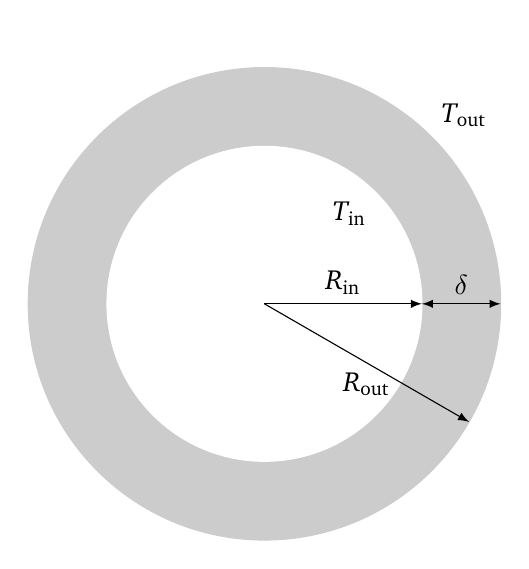
\begin{tikzpicture}
       \draw[dashed,white] (0,-3) -- (0,3.5);
       \filldraw[black!20!white] (0,0) circle [radius=3cm];
       \filldraw[white] (0,0) circle [radius=2cm];
       \draw[->] (0,0) -- node[midway,above]{$R_\text{in}$}(0:2cm);
       \draw[->] (0,0) -- node[midway,below]{$R_\text{out}$}(-30:3cm);
       \draw[<->] (0:2cm) -- node[midway,above]{$\delta$} (0:3cm);
       \node[anchor=north east] at (45:2cm) {$T_\text{in}$};
       \node[anchor=south west] at (45:3cm) {$T_\text{out}$};
      \end{tikzpicture}
      \caption{\label{fig:Tdr_esfera_hueca}Schematic representation of a hollow sphere with the representative parameters used to derive the thermal flux from the internal surface to the external surface through the volume enclosed by both surfaces.}
\end{figure}

Let us consider the temperature profile inside the thermal boundary layers. To this end, we will derive the temperature distribution across a hollow sphere assuming that heat flows radially outwards. As it is shown in Figure~\ref{fig:Tdr_esfera_hueca}, $R_\text{in}$ and $R_\text{out}$ are the radii of the inner and outer spherical surfaces, respectively. The former is assumed to be at the temperature $T_\text{in}$, while the latter is at the temperature $T_\text{out}$, with $T_\text{in} > T_\text{out}$. The thickness of the hollow sphere is $\delta = R_\text{out} - R_\text{in}$. First, we will make use of the continuity equation in its differential form:
\begin{equation}
      \label{ec:continuity_eq_diff}
      \pdiff{u}{t} + \nabla \cdot \vec{q} = 0.
\end{equation} As can be noted, we neglect heat sources within the considered layer. The next step is to consider the steady state heat flow. In that case, we have that:
\begin{equation}
      \label{ec:cont_eq_energy_steady}
      \nabla \cdot \vec{q} = 0.
\end{equation} At this point it arises the question about the validity of this approach since we are considering time evolution of the internal temperatures of the Earth. However, as is pointed out by \citet{stamenkovicetal2012}, the aforementioned approximation can be justified by the fact that relaxation time of the lithosphere is typically on the order of 100 Ma. In contrast, the relaxation time of the mantle is of the order of few Ga, in other words, the latter is much grater that the former. 

Since we assume that heat flows radially outwards, then the heat flux vector is given by:
\begin{equation}
      \vec{q} = q_r \hat{\vec{r}},
\end{equation} where $\hat{\vec{r}}$ is the corresponding unit vector that is perpendicular to the spherical surfaces at each point and its sense is outwards the aforementioned surface. Taking this assumption into account, Equation~\eqref{ec:cont_eq_energy_steady} can be rewritten as:
\begin{equation}\label{ec:dqrdr}
      \frac{1}{r^2} \frac{\text{d}}{\text{d} r} \left[r^2 \, q_r (r) \right] = 0.
\end{equation} On the other hand, as we have assumed that heat is transported by conduction across the layer, the relationship between the heat flux and temperature is given by the Fourier law:
\begin{equation}
      \label{ec:fourier_law_gen}
      \vec{q} = - \, k \, \nabla T.
\end{equation} If we assume that temperature depends only on the radial distance:
\begin{equation}
      \label{ec:fourier_law_r}
      q_r = - \, k \, \frac{\text{d} T}{\text{d} r}.
\end{equation} Then, by inserting Equation~\eqref{ec:fourier_law_r} into Equation~\eqref{ec:dqrdr} and simplifying we obtain:
\begin{equation}
      \label{ec:d2Trdr2}
      \fdiff{}{r} \left[r^2 \, \fdiff{T (r)}{r} \right] = 0.
\end{equation} The solution of Equation~\eqref{ec:d2Trdr2} considering the boundary conditions $T(R_\text{in}) = T_\text{in}$ and $T (R_\text{out}) = T_\text{out}$ is \citep{carslaw_jaeger_1959}:
\begin{equation}
      \label{ec:Tdr_hollow}
      T_\text{cond} (r) = \frac{R_\text{out} \, T_\text{out} \left(r - R_\text{in}\right) + R_\text{in} T_\text{in} \left(R_\text{out} - r\right)}{\left(R_\text{out} - R_\text{in}\right) r}.
\end{equation} In the latter equation, we added the subscript ``cond'' to stress the fact that this expression is valid for conductive heat flow.

Now we move our attention to the adiabatic temperature distribution. In general terms, such temperature profile satisfies \citep{turcotte2014}:
\begin{equation}
      \label{ec:adiabatic_TdP}
      \fdiff{T}{P} = \frac{\alpha \, T}{\rho \, c},
\end{equation} were $P$ is the pressure. In principle, Equation~\eqref{ec:adiabatic_TdP} cannot be solved directly because physical properties, such as $\alpha$, $\rho$, and $c$, of both the core and mantle varies with depth \citep[see e.g.][]{valenciaetal2006}. In the case of the core we consider the expression given by \citet{stevensonetal1983}:
\begin{equation}
    \label{ec:Tc_r_adia}
    T_\text{c} (r) = T_\textsc{cmb} \left[\frac{1 + T_{a,1} \, P (r) + T_{a,2} \, P^2 (r)}{1 + T_{a,1} \, P_\textsc{cmb} + T_{a,2} \, P_\textsc{cmb}^2}\right],
\end{equation} where $P_\textsc{cmb}$ is the pressure at the CMB, i.e. $P_\textsc{cmb} = P \left(R_\text{c}\right)$, while $T_{a,1}$ and $T_{a,2}$ are constants. The expression of the pressure as a function of the radial distance $r$ is obtained by fitting the PREM data \citep{PREM1981} to a quadratic polynomial:
\begin{equation}
    \label{ec:Pdr}
    P(r) = \begin{cases}
        367.767 - 0.0144178 \, r - 1.52163 \E{-5} \, r^2, & \text{ if } 0 \leq r \leq R_\text{c} \\
        397.012 - 0.0901277 \, r + 4.35256 \E{-6} \, r^2, & \text{ if } R_\text{c} \leq r \leq R_\oplus
    \end{cases}
\end{equation} where $P$ is given in GPa and $r$ in km.

Equation~\eqref{ec:adiabatic_TdP} can be transformed into a differential equation in which the independent variable is the radial distance by assuming hydrostatic equilibrium:
\begin{equation}
      \label{ec:hidrostatic_eq}
      \fdiff{P}{r} = - \, \rho \, g.
\end{equation} Then, we arrive to:
\begin{equation}
      \label{ec:adiabatic_Tdr}
      \fdiff{T}{r} = \frac{\alpha \, T}{\rho \, c} \fdiff{P}{r} = - \frac{\alpha \, g \, T}{c}.
\end{equation} If we assume that the physical properties $\alpha$, $g$, and $c$ are constant, then the Equation~\eqref{ec:adiabatic_Tdr} can be solved straightforwardly:
\begin{equation}
    \label{ec:Tdr_adiabatic_gen}
    T (r) = A \, \exp \left(-\frac{\alpha \, g \, r}{c}\right),
\end{equation} where $A$ is a constant to be determined by the initial conditions. For example, by setting the general condition that the temperature is $T_0$ at the radial distance $R_0$, then:
\begin{equation}
    \label{ec:Tdr_IC}
    T (R_0) = T_0 = A \, \exp \left(-\frac{\alpha \, g \, R_0}{c}\right),
\end{equation} and consequently:
\begin{equation}
    \label{ec:Tdr_adiabatic_0}
    T (r) = T_0 \, \exp \left[\frac{\alpha \, g}{c} \left(R_0 - r\right)\right],
\end{equation} where $T_0$ can be thought as a reference temperature. When the expression given by Equation~\eqref{ec:Tdr_adiabatic_0} is evaluated at some particular value of $r$, $T$ is known as the \emph{potential temperature} \citep{mckenzie_bickle_1988}, $T_\text{pot}$. Thus, the potential temperature is the temperature a mass element would have if it were taken from that particular radius to the reference one.

Is of particular interest in the study of the mantle's thermal evolution to take as reference the temperature at the base of the upper thermal boundary layer. Thus:
\begin{equation}
    \label{ec:Tdr_adiabatic_ubl}
    T (r) = T_\textsc{ubl} \, \exp \left[\frac{\alpha \, g}{c} \left(R_\oplus - \delta_\textsc{ubl} - r\right)\right].
\end{equation} The simplest way to compute the potential temperature is at the Earth's surface ($r = R_\oplus$), where it could be easily measured. In consequence:
\begin{equation}
    \label{ec:Tpot}
    T_\text{pot} = T_\textsc{ubl} \, \exp \left(- \frac{\alpha \, g \, \delta_\textsc{ubl}}{c}\right).
\end{equation}

Concerning the temperature profile within mantle, but outside the thermal boundary layers, it is well approximated by a linear expression because mantle the adiabatic scale length is much larger than mantle thickness \citep{driscollybarnes2015}. Thus, by expanding Equation~\eqref{ec:Tdr_adiabatic_ubl} in power series and retaining up to the linear term, we arrive to:
\begin{equation}
    \label{ec:Tdr_adiabatic_linear}
    T_\text{m} (r) \approx T_\textsc{ubl} + \frac{\alpha_\text{m} \, g_\text{m} \, T_\textsc{ubl}}{c_\text{m}} \left(R_\oplus - \delta_\textsc{ubl} - r\right).
\end{equation}

Finally, the expression of the temperature profile inside the Earth is given by:
\begin{equation}
    \label{ec:Tdr_earth}
    T (r) = \begin{cases}
        T_\textsc{cmb} \left[\dfrac{1 + T_{a,1} \, P (r) + T_{a,2} \, P^2 (r)}{1 + T_{a,1} \, P_\textsc{cmb} + T_{a,2} \, P_\textsc{cmb}^2}\right] & \text{ if } 0 \leq r \leq R_\text{c} \\
         & \\
        \dfrac{\left(R_\text{c} + \delta_\textsc{lbl}\right) \, T_\textsc{lbl} \left(r - R_\text{c}\right) + R_\text{c} T_\textsc{cmb} \left(R_\text{c} + \delta_\textsc{lbl} - r\right)}{\delta_\textsc{lbl} \, r} & \text{ if } R_\text{c} \leq r \leq R_\text{c} + \delta_\textsc{lbl} \\
        & \\
        T_\textsc{ubl} + \dfrac{\alpha_\text{m} \, g_\text{m} \, T_\textsc{ubl}}{c_\text{m}} \left(R_\oplus - \delta_\textsc{ubl} - r\right) & \text{ if } R_\text{c} + \delta_\textsc{lbl} \leq r \leq R_\oplus - \delta_\textsc{ubl} \\
        & \\
        \dfrac{R_\oplus \, T_\text{s} \left(r - R_\oplus + \delta_\textsc{ubl}\right) + \left(R_\oplus - \delta_\textsc{ubl}\right) T_\textsc{ubl} \left(R_\oplus - r\right)}{\delta_\textsc{ubl} \, r} & \text{ if } R_\oplus - \delta_\textsc{ubl} \leq r \leq R_\oplus.
    \end{cases}
\end{equation} By virtue of Equation~\eqref{ec:Tdr_adiabatic_linear}, and taking into account Figure~\ref{fig:Tdr_manto}, we can note that the temperature at the top of the lower thermal boundary layer can be computed by \citep{grottybreuer2008}:
\begin{equation}
      \label{ec:T_lbl}
      T_\textsc{lbl} = T_\textsc{ubl} + \frac{\alpha_\text{m} \, g_\text{m} \, T_\textsc{ubl}}{c_\text{m}} \left(R_\oplus - \delta_\textsc{ubl} - R_\text{c} - \delta_\textsc{lbl}\right).
\end{equation} Thus, we can conclude that the temperature profile of the Earth's interior is fully characterized by the surface temperature, $T_\text{s}$, the temperature at the base of the upper thermal boundary layer, $T_\textsc{ubl}$, and the temperature at the core-mantle boundary, $T_\textsc{cmb}$.

\subsection{Mantle viscosity\label{ss:matle_visc}}

The dynamic viscosity, $\eta$, of the mantle depends, in general terms, on the temperature ($T$) and pressure ($P$) \citep{valenciaetal2006,henningetal2009,stamenkovicetal2012}. The functional form of this dependence is usually expressed in the form of Arrhenius' law:
\begin{equation}
      \label{ec:visc_arrhen}
      \eta (T,P) = b \exp \left(\frac{E^\ast + P \, V_\text{eff}^\ast}{R_\text{gas} T}\right),
\end{equation} where $b$ is a constant, $E^\ast$ and $V_\text{eff}^\ast$ are the energy and effective volume of activation, respectively, and $R_\text{gas}$ is the Universal constant of ideal gases.

As can be seen in Equation~\eqref{ec:visc_arrhen}, the activation energy describes the coupling between viscosity and temperature, while the effective activation volume describes the coupling between pressure and viscosity. For reasons of simplicity, only the dependence of viscosity on temperature will be considered. In this sense, we set $V_\text{eff}^\ast = 0$ and, consequently, Equation~\eqref{ec:visc_arrhen} is written as:
\begin{equation}
      \label{ec:visc_arrhen_T}
      \eta (T) = b \exp \left(\frac{E^\ast}{R_\text{gas} T}\right).
\end{equation} Following \citet{stamenkovicetal2012}, the latter equation can be rewritten in a more convenient way by considering a viscosity reference value corresponding to a temperature reference value, i.e. $\eta_\text{ref} = \eta (T_\text{ref})$. In this way the constant $b$ can be eliminated and Eq~\eqref{ec:visc_arrhen_T} becomes:
\begin{equation}
      \label{ec:visc_T_Tref}
      \eta (T) = \eta_\text{ref} \exp \left[\frac{E^\ast}{R_\text{gas}} \left(\frac{1}{T} - \frac{1}{T_\text{ref}}\right)\right].
\end{equation}

\subsection{Expression of the heat fluxes}

As we have pointed out before, heat is transported by conduction across each thermal boundary layer, thus the corresponding heat flux ($q$) for each boundary layer is given by:
\begin{equation}
    \label{ec:heat_flux_gen}
    q = k_\text{m} \frac{\Delta T}{\delta},
\end{equation} where $k_\text{m}$ is the thermal conductivity, which is considered constant for the whole mantle, $\Delta T$ is the temperature jump across the corresponding boundary layer of thickness $\delta$. The thickness of the upper thermal boundary layer is obtained by virtue of the Nu-Ra relationship \citep{schubertetal2001}:
\begin{equation}
    \label{ec:delta_ubl}
    \delta_\textsc{ubl} = \left(R_\oplus - R_\text{c}\right) \left(\frac{\text{Ra}_\text{cr}}{\text{Ra}}\right)^\beta,
\end{equation} where $\beta$ is a real exponent. The thickness of the lower thermal boundary layer ($\delta_\textsc{lbl}$) is expected to be thinner than $\delta_\textsc{ubl}$ because of the aforementioned strong dependence of the viscosity on the temperature. For this reason $\delta_\textsc{lbl}$ is computed locally \citep{stevensonetal1983}:
\begin{equation}
    \label{ec:delta_lbl}
    \delta_\textsc{lbl} = \left[\frac{ \text{Ra}_\text{cr}^\text{(cmb)} \kappa \, \eta_\textsc{lbl} }{g \, \alpha_\text{m} \, \Delta T_\textsc{lbl}}\right]^{1/3},
\end{equation} where $\text{Ra}_\text{cr}^\text{(cmb)}$ is the local critical Rayleigh number at the CMB and the viscosity is evaluated at the mean temperature within the lower thermal boundary layer:
\begin{equation}
    \label{ec:visc_lbl}
    \eta_\textsc{lbl} = \eta \left(\frac{T_\textsc{lbl} + T_\textsc{cmb}}{2}\right).
\end{equation} In consequence, we have:
\begin{align}
    \label{ec:Q_cmb_Q_conv}
    \dot{Q}_\text{conv} &= A_\oplus \, k_\text{m} \frac{\Delta T_\textsc{ubl}}{\delta_\textsc{ubl}} = A_\oplus \, k_\text{m} \frac{\left(T_\textsc{ubl} - T_\text{s}\right)}{\delta_\textsc{ubl}} \\
    \dot{Q}_\textsc{cmb} &= A_\text{c} \, k_\text{m} \frac{\Delta T_\textsc{lbl}}{\delta_\textsc{lbl}} = A_\text{c} \, k_\text{m} \frac{\left(T_\textsc{cmb} - T_\textsc{lbl}\right)}{\delta_\textsc{lbl}} \\
\end{align}

\subsection{Inner core growth}

Formerly, we mentioned that the inner core grows by precipitation of heavy elements as the core cools down. This phenomenon gives raise to the second term on the left hand side of Equation~\eqref{ec:dTmdt_core_gral}. In order to compute the time derivative of the inner core mass, we can express it as:
\begin{equation}
    \label{ec:Mic}
    M_\text{ic} = \frac{4}{3} \pi \, \rho_\text{c} \, R_\text{ic}^3,
\end{equation} where $\rho_\text{c}$ is the mean density of the core, considered constant, and $R_\text{ic}$ is the inner core radius, which is given by \citep{stevensonetal1983}:
\begin{equation}
    \label{ec:Ric}
    R_\text{ic} = \sqrt{\frac{2 \left(P_{\text{c},\oplus} - P_\text{io}\right) R_\text{c}}{\rho_\text{c} \, g}},
\end{equation} where $P_{\text{c},\oplus}$ and $P_\text{io}$ are the pressures at the Earth's centre and at the inner-outer core boundary, respectively. $P_\text{io}$ is determined by the intersection between the adiabatic temperature profile within the core and the corresponding liquidus temperature profile:
\begin{equation}
    \label{ec:T_liq_c}
    T_\text{liq,c} (r) = T_{\text{liq,c},0} \left(1 - 2 \, \chi \right) \left[1 + T_{\text{liq,c},1} \, P (r) + T_{\text{liq,c},2} \, P^2 (r)\right],
\end{equation} where $\chi$ is the fraction of light elements dissolved in the core, which tend to lower the liquidus temperature, while $T_{\text{liq,c},1}$ and $T_{\text{liq,c},2}$ are constants. By virtue of the conservation of mass of these light elements, we obtain:
\begin{equation}
    \label{ec:chi_chi0}
    \chi = \frac{\chi_0 \, R_\text{c}^3}{R_\text{c}^3 - R_\text{ic}^3},
\end{equation} where $\chi_0$ is the initial concentration of the light elements. Then, taking into account that $P \left(R_\text{io}\right) = P_\text{io}$, it is satisfied that $T_\text{c} \left(R_\text{io}\right) = T_\text{liq,c} \left(R_\text{io}\right)$, that is:
\begin{equation}
    \label{ec:Pio}
    T_\textsc{cmb} \left[\frac{1 + T_{a,1} \, P_\text{io} + T_{a,2} \, P_\text{io}^2}{1 + T_{a,1} \, P_\textsc{cmb} + T_{a,2} \, P_\textsc{cmb}^2}\right] = T_{\text{liq,c},0} \left(1 - 2 \, \chi \right) \left[1 + T_{\text{liq,c},1} \, P_\text{io} + T_{\text{liq,c},2} \, P_\text{io}^2 \right],
\end{equation} from which the value of $P_\text{io}$ can be found. By defining the constant
\begin{equation}
    \label{ec:def_xi}
    \xi = T_{\text{liq,c},0} \left(1 - 2 \, \chi\right) \left(1 + T_{a,1} \, P_\textsc{cmb} + T_{a,2} \, P_\textsc{cmb}^2\right)
\end{equation} one can rewrite Eq.~\eqref{ec:Pio} as a quadratic equation:
\begin{equation}
    \label{ec:Pio_cuad}
    \left(T_\textsc{cmb} (t) - \xi\right) + \left(T_\textsc{cmb} (t) \, T_{a,1} - \xi \, T_{\text{liq,c},1}\right) P_\text{io} + \left(T_\textsc{cmb} (t) \, T_{a,2} - \xi \, T_{\text{liq,c},2}\right) P_\text{io}^2 = 0.
\end{equation} This equation defines $P_\text{io}$ as an implicit function of time, which must be taken into account when calculating the derivative of $M_\text{ic}$ with respect to time, since the inner core radius varies in time because it depends on $P_\text{io}$.

In order to calculate the time derivative of the inner core mass, we must to take into account that $R_\text{ic}$ is a function of time through $P_\text{io}$ and that, in its turn, $P_\text{io}$ depends also on time through $T_\textsc{cmb}$, as can be noted from Equation~\eqref{ec:Pio_cuad}. Then, by virtue of Equation~\eqref{ec:Mic}, we have:
\begin{equation}
    \label{ec:dmicdt_gen}
    \fdiff{M_\text{ic}}{t} = 4 \, \pi \, \rho_\text{c} \, R_\text{ic}^2 \fdiff{R_\text{ic}}{t}.
\end{equation} According to what we pointed out before, the time derivative of the inner core radius can be expressed as:
\begin{equation}
      \label{ec:dRicdt}
      \fdiff{R_\text{ic}}{t} = \fdiff{R_\text{ic}}{P_\text{io}} \fdiff{P_\text{io}}{t},
\end{equation} and the time derivative of the pressure at the inner-outer core boundary as:
\begin{equation}
    \label{ec:dPiodt}
    \fdiff{P_\text{io}}{t} = \fdiff{P_\text{io}}{T_\textsc{cmb}} \fdiff{T_\textsc{cmb}}{t},
\end{equation} where:
\begin{equation}
      \label{ec:dRicdPio}
      \fdiff{R_\text{ic}}{P_\text{io}} = - \frac{R_\text{c}}{\rho_\text{c} \, g \, R_\text{ic}}
\end{equation}
\begin{equation}
    \label{ec:dPiodTcmb}
    \fdiff{P_\text{io}}{T_\textsc{cmb}} = \frac{\left(1 + T_{a,1} \, P_\text{io} + T_{a,2} \, P_\text{io}^2\right)}{\left[\xi \left(T_{\text{liq,c},1} + 2 \, T_{\text{liq,c},2} \, P_\text{io}\right) - T_\textsc{cmb} \left(T_{a,1} + 2 \, T_{a,2} \, P_\text{io}\right)\right]}.
\end{equation} Finally, we arrive to:
\begin{equation}
      \label{ec:dMicdt}
      \fdiff{M_\text{ic}}{t} = - \frac{A_\text{c} \, R_\text{ic}}{g \, R_\text{c}} \fdiff{P_\text{io}}{T_\textsc{cmb}} \fdiff{T_\textsc{cmb}}{t},
\end{equation} where $A_\text{c}$ is the outer core surface area.

\subsection{Partial melt within the mantle}

Now let us consider the second term on the left hand side of Equation~\eqref{ec:dTmdt_mantle_gral}, more precisely the calculation of the time derivative of the mass of melted materials in the mantle.

In order to estimate the mass of melted materials within mantle, we can make use of the concept of mean mantle melt fraction ($\valmed{\phi}_\text{m}$), which is defined as the ratio between $M_\text{melt}$ to the mass of the mantle, i.e.:
\begin{equation}
    \valmed{\phi}_\text{m} = \frac{M_\text{melt}}{M_\text{m}}.
\end{equation} The convenience of this concept is that $\valmed{\phi}_\text{m}$ can be computed as the volume averaged \emph{local melt fraction}, which is assumed to be a function of the radial distance only. Thus:
\begin{equation}
    \label{ec:fmeltm}
    \valmed{\phi}_\text{m} = \frac{1}{V_\text{m}} \iiint\limits_{V_\text{m}} \phi(r) \, \text{d} V,
\end{equation} where $V_\text{m}$ is the mantle volume and  $\phi (r)$ is given by:
\begin{equation}
    \label{ec:melt_frac}
    \phi (r) = \frac{T(r) - T_\text{sol} (r)}{T_\text{liq} (r) - T_\text{sol} (r)}.
\end{equation} Here, $T_\text{sol} (r)$ and $T_\text{liq} (r)$ are the mantle solidus and liquidus temperature profiles, respectively. In our model we consider the corresponding expressions given by \citet{monteuxetal2016}:
\begin{align}
    T_\text{sol} (r) = 
    \begin{cases}
    1661.2 \left( \frac{P(r)}{1.336} + 1\right)^{\frac{1}{7.437}} & \text{ si } P \leq 20 \, \text{GPa} \\
    2081.8 \left( \frac{P(r)}{101.69} + 1\right)^{\frac{1}{1.226}} & \text{ si } P \geq 20 \, \text{GPa} 
    \end{cases}
\end{align}
\begin{align}
    T_\text{liq} (r) =
    \begin{cases}
    1982.1 \left( \frac{P(r)}{6.594} + 1\right)^{\frac{1}{5.374}} & \text{ si } P \leq 20 \, \text{GPa} \\
    2006.8 \left( \frac{P(r)}{34.65} + 1\right)^{\frac{1}{1.844}} & \text{ si } P \geq 20 \, \text{GPa},
    \end{cases}
\end{align} where $r$ is expressed in kilometers and the pressure in GPa, in consistece with the expression of $P(r)$, given by Equation~\eqref{ec:Pdr}.



\subsection{Final expression of the fundamental equations}

\subsection{Heat sources}

In agreement with what we have pointed out in Sections~\ref{sec:intro} and \ref{sec:theory}, two sources of heat are considered in our model, namely the heat generated by the decay of radioactive elements and that of tidal origin, which is associated with the non-elastic behavior of mantle materials undergoing tidal stress. In our model, the deformation of the Earth due to the gravitational attraction from the Moon is allowed for.

\subsubsection{Decay of radioactive isotopes}

The modeling of this kind of sources is given by \citet{driscollybercovici2014} for the core and by \citet{turcotte2014} for the mantle. The former has the following simple exponential form:
\begin{equation}
    \label{ec:Qradc}
    \dot{Q}_\text{rad,c} = \dot{Q}_{\text{rad,c},0} \exp \left(- \frac{t}{\tau_\text{rad,c}}\right),
\end{equation} where $\dot{Q}_{\text{rad,c},0}$ is the rate of radiogenic heat production at $t=0$ and $\tau_\text{rad,c}$ is the radioactive decay time scale.

The radiogenic heat production rate in the mantle takes into account the decay of the most thermally relevant isotopes Uranium (235 and 238), Thorium and Potassium, and is given by:
\begin{equation}
    \label{ec:Qradm}
    \dot{Q}_\text{rad,m} = M_\text{m} \, H(t),
\end{equation} where $H(t)$ is the radiogenic heat production rate per unit mass and is expressed as:
\begin{multline}
    \label{ec:Hdt_tot}
    H (t) = 0.9928 \, C_0^{\text{U}} H_0 \left(^{238}\mbox{U}\right) \exp \left[- \frac{\ln 2}{\tau_{\frac{1}{2}} \left(^{238}\mbox{U}\right)} (t - t_0) \right] + 0.0071 \, C_0^{\text{U}} H_0 \left(^{235}\mbox{U}\right) \exp \left[- \frac{\ln 2}{\tau_{\frac{1}{2}}\left(^{235}\mbox{U}\right)} (t - t_0) \right] \\ + C_0^{\text{Th}} H_0 \left(^{232}\mbox{Th}\right) \exp \left[- \frac{\ln 2}{\tau_{\frac{1}{2}} \left(^{232}\mbox{Th}\right)} (t - t_0) \right] + 1.19 \times 10^{-4} C_0^{\text{K}} H_0 \left(^{40}\mbox{K}\right) \exp \left[- \frac{\ln 2}{\tau_{\frac{1}{2}} \left(^{40}\mbox{K}\right)} (t - t_0) \right].
\end{multline} where $C_0$ and $H_0$ are the concentration and heat production rate per unit mass of each isotope at instant $t_0$, while $\tau_\frac{1}{2}$ is the corresponding half-life.

\subsubsection{Tidal heating}

Concerning the tidal heating source, the corresponding heat production rate is given by:
\begin{equation}
    \label{ec:Qtidal}
    \dot{Q}_\text{tidal} = f_\text{tvf} \, \valmed{P}_\oplus^\text{tide}
\end{equation} where $\left\langle P \right\rangle_\text{m}^\text{tide}$ is the mean tidal heating rate in the Earth's mantle. The formula that we will use to compute the aforementioned quantity was developed by \citet{efromak2014}. However, that formula gives the mean tidal heating rate over the whole volume of the considered body, the Earth in our case. However, for terrestrial planets most tidal dissipation occurs within the mantle \citep{henningyhurford2014}. In order to overcome this caveat, we follow the work by \citep{renaudhenning2018} by defining the tidal volume factor, $f_\text{tvf}$, as:
\begin{equation}
    \label{ec:ftvf}
    f_\text{tvf} = \frac{R_\phi^3 - R_\text{c}^3}{R_\oplus^3},
\end{equation} where $R_\phi$ is the distance from the center of the Earth where the melt fraction ($\phi$) is equal to the disaggregation point $\phi_\textsc{d}$, which is a critical value of the melt fraction above which mantle material cannot behave as a solid any more. $\left\langle P \right\rangle_\oplus^\text{tide}$ is given by:
\begin{multline}\label{ec:potdis_mareas}
      \left\langle P \right\rangle_\oplus^\text{tide} = \frac{G \, M_{\leftmoon}^2}{a} \sum_{l=2}^\infty \left(\frac{R_\oplus}{a}\right)^{2l+1} \sum_{m=0}^l \frac{(l-m)!}{(l+m)!} \left(2-\delta_{0m}\right) \\ \times \sum_{p=0}^l F_{lmp}^2 (i) \sum_{q=-\infty}^{\infty} G_{lpq}^2 (e) \, \omega_{lmpq} \, K_{\text{I}} \left(l,\omega_{lmpq}\right),
\end{multline} where $G$ is the gravitation constant, $M_{\leftmoon}$ is the mass of the Moon, $R_\oplus$ is the mean Earth radius, $a$ is the major semiaxis, $\delta_{0m}$ is the Kronecker delta distribution, $F_{lmp} (i)$ and $G_{lpq} (e)$ are the inclination \citep{goodwagner2008} and eccentricity \citep{giacaglia1976b} functions, respectively.

The factor $K_\text{I} \left(l,\omega_{lmpq}\right)$ describes the rheological response of Earth, i.e. the modification of its gravitational field due to the deformation caused by the gravitational attraction forces exerted by the Moon, and is given by:
\begin{equation}\label{ec:imklJ} 
      K_\text{I} (l,\omega_{lmpq}) = - \frac{3}{2} \frac{1}{l-1} \frac{B_l \, \Im \left[\bar{J} (\chi) \right] \sgn \left(\omega_{lmpq} \right)}{\left(\Re \left[ \bar{J} (\chi) \right] + B_l \right)^2 + \left(\Im \left[ \bar{J} (\chi) \right]\right)^2}, 
\end{equation} where $\Re \left(\bar{z}\right)$ and $\Im \left(\bar{z}\right)$ are the real and imaginary parts of the complex number $\bar{z}$, respectively, and $\chi_{lmpq}$ are the physical tidal frequencies which are defined through:
\begin{equation}
      \label{ec:def_chi_lmpq}
      \chi_{lmpq} = \left\vert \omega_{lmpq} \right\vert,
\end{equation} where the tidal modes $\omega_{lmpq}$ are given by:
\begin{equation}\label{ec:def_wlmpq}
      \omega_{lmpq} = (l-2p) \, \dot{\omega} + (l-2p+q) \, \dot{\mathcal{M}} + m \left(\dot{\ascnode} - \dot{\theta}\right),
\end{equation} where $\dot{\mathcal{M}}$, $\dot{\omega}$ and $\dot{\ascnode}$ are the time rates of the mean anomaly $\mathcal{M}$, the argument of perigee $\omega$ and the longitude of ascending node $\ascnode$ \citep{efroimsky2012,efroimsky2015}. The latter two angles, as well as the inclination of the Moon's orbital plane $i$, are defined with respect to the Earth's equatorial plane. In many applications $\dot{\omega} \approx 0$ and $\dot{\ascnode} \approx 0$ while $\dot{\mathcal{M}} \approx n$. Consequently the approximation 
\begin{equation}
      \label{ec:wlmpq_aprox}
      \omega_{lmpq} \approx (l-2p+q) \, n - m \, \dot{\theta},
\end{equation} is generally valid and frequently used in the specialized literature. In Equation~\eqref{ec:wlmpq_aprox}, $n$ is the mean orbital frequency which for the unperturbed two-body problem is defined by the mathematical expression of Kepler's third law:
\begin{equation}
      \label{ec:defn}
      G \left(M_{\oplus} + M_{\leftmoon}\right) = n^2 a^3,
\end{equation} where $M_\oplus$ is the mass of the Earth. In addition, $B_l$ is given by:
\begin{equation}
      \label{ec:defBl}
      B_l = \frac{R_\oplus \left(2 l^2 + 4 l + 3\right)}{l \, G \, M_\oplus \, \rho_\oplus},
\end{equation} where $\rho_\oplus$ is the mean density of the Earth. Lastly, $\bar{J} (\chi)$ is the complex creep-response or complex compliance function \citep{efroimsky2012,efroimsky2015}, which is defined through:
\begin{equation}\label{ec:defJcomplex} 
      \bar{J} (\chi) = \int_0^\infty \dot{J} (t-t') \exp{\left[- \text{i} \chi (t-t')\right]} \, 
      \text{d}t',
\end{equation} where the over-dot means differentiation with respect to $t'$ and $\text{i} = \sqrt{-1}$ is the imaginary unit. The particular form of the kernel $J(t-t')$ depends on the particular rheological model considered. However, it is generally given by:
\begin{equation}\label{ec:kernJgral} 
      J (t-t') = J(0) \, \Theta (t-t') + \mbox{viscous and hereditary terms},
\end{equation} where $J(0)$ is the instantaneous value of the compliance which, in its turn, is the reciprocal value of the instantaneous rigidity $\mu (0)$, and $\Theta (t-t')$ is the Heaviside step function \citep{efroimsky2012}.

\subsubsection{Rheological models}

The first term on the right hand side of Equation~\eqref{ec:kernJgral} describes the instantaneous elastic response in deformation of the body under stress. However, the general rheological response of a real solid body is a mixture of elastic and anelastic behavior. The latter includes viscous and hereditary behaviors.

The complex compliance is obtained from the \emph{constitutive equation}, which relates stress and strain. In a linear medium, assumed to be homogeneous, incompressible and isotropic, the relationship between the components of the stress tensor and the strain tensor is, in general terms, given by:
\begin{equation}\label{ec:ecconstfrec} 
      2 \, \bar{u}_{\gamma \nu} (\chi) = \bar{J} (\chi) \, \bar{\sigma}_{\gamma \nu} (\chi),
\end{equation} where $\bar{u}_{\gamma \nu} (\chi)$ and $\bar{\sigma}_{\gamma \nu} (\chi)$ are the complex counterparts of the strain and stress tensors, respectively \citep{efroimsky2012}.

\begin{figure}[t]
 \centering      
 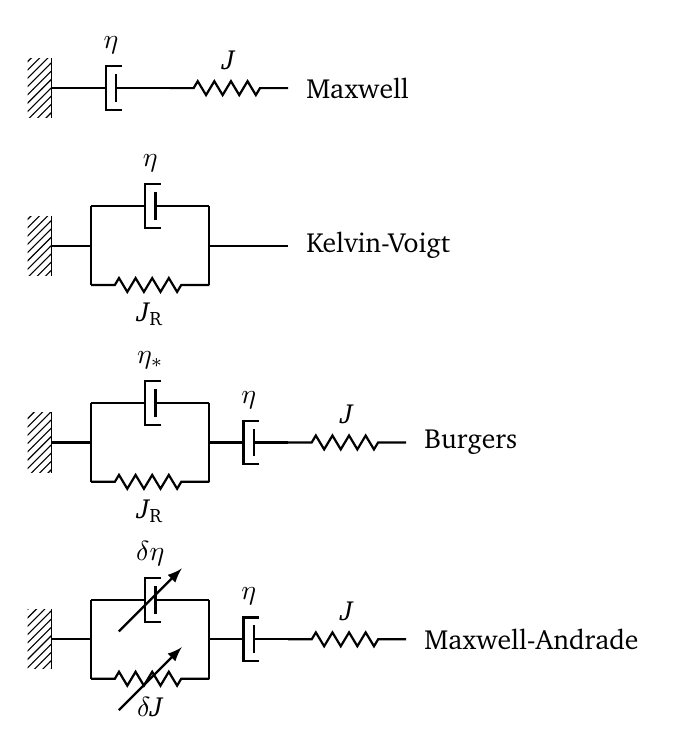
\begin{tikzpicture}
      \tikzstyle{spring}=[thick,decorate,decoration={zigzag,pre length=0.3cm,post length=0.3cm,segment length=6}]
      \tikzstyle{damper}=[thick,decoration={markings,  
      mark connection node=dmp,
      mark=at position 0.5 with 
      {
      \node (dmp) [thick,inner sep=0pt,transform shape,rotate=-90,minimum width=15pt,minimum height=3pt,draw=none] {};
      \draw [thick] ($(dmp.north east)+(2pt,0)$) -- (dmp.south east) -- (dmp.south west) -- ($(dmp.north west)+(2pt,0)$);
      \draw [thick] ($(dmp.north)+(0,-5pt)$) -- ($(dmp.north)+(0,5pt)$);
      }
      }, decorate]
      \tikzstyle{ground}=[fill,pattern=north east lines,draw=none,minimum width=0.75cm,minimum height=0.3cm]
      %%% Maxwell
      \node (ground1) at (0,7) [ground,anchor=north,rotate=-90] {};
      \draw (ground1.north west) -- (ground1.north east);
      \draw[damper] (0,7) -- node[midway,above,yshift=+0.3cm]{$\eta$} (1.5,7);
      \draw[spring] (1.5,7) -- node[midway,above,yshift=+0.1cm]{$J$} (3,7) node[anchor=west,xshift=0.1cm]{Maxwell};
      %%%% Kelvin-Voigt
      \node (ground1) at (0,5) [ground,anchor=north,rotate=-90] {};
      \draw (ground1.north west) -- (ground1.north east);
      \draw[thick] (0,5) -- (0.5,5);
      \draw[thick] (0.5,5.5) -- (0.5,4.5);
      \draw[damper] (0.5,5.5) -- node[midway,above,yshift=+0.3cm]{$\eta$} (2,5.5);
      \draw[spring] (0.5,4.5) -- node[midway,below,yshift=-0.1cm]{$J_\text{R}$} (2,4.5);
      \draw[thick] (2,5.5) -- (2,4.5);
      \draw[thick] (2,5) -- (3,5) node[anchor=west,xshift=0.1cm]{Kelvin-Voigt};
      %%%% Burgers
      \node (ground1) at (0,2.5) [ground,anchor=north,rotate=-90] {};
      \draw (ground1.north west) -- (ground1.north east);
      \draw[thick] (0,2.5) -- (0.5,2.5);
      \draw[thick] (0.5,3) -- (0.5,2);
      \draw[damper] (0.5,3) -- node[midway,above,yshift=+0.3cm]{$\eta_{\ast}$} (2,3);
      \draw[spring] (0.5,2) -- node[midway,below,yshift=-0.1cm]{$J_\text{R}$} (2,2);
      \draw[thick] (2,3) -- (2,2);
      \draw[damper] (2,2.5) -- node[midway,above,yshift=+0.3cm]{$\eta$} (3,2.5);
      \draw[spring] (3,2.5) -- node[midway,above,yshift=+0.1cm]{$J$} (4.5,2.5) node[anchor=west,xshift=0.1cm]{Burgers};
      %%%% Maxwell-Andrade
      \node (ground1) at (0,0) [ground,anchor=north,rotate=-90] {};
      \draw (ground1.north west) -- (ground1.north east);
      \draw[thick] (0,0) -- (0.5,0);
      \draw[thick] (0.5,0.5) -- (0.5,-0.5);
      \draw[damper] (0.5,0.5) -- node[midway,above,yshift=+0.3cm]{$\delta \eta$} (2,0.5);
      \draw[thick,->] (0.85,0.1) -- (1.65,0.9);
      \draw[spring] (0.5,-0.5) -- node[midway,below,yshift=-0.1cm]{$\delta J$} (2,-0.5);
      \draw[thick,->] (0.85,-0.9) -- (1.65,-0.1);
      \draw[thick] (2,0.5) -- (2,-0.5);
      \draw[damper] (2,0) -- node[midway,above,yshift=+0.3cm]{$\eta$} (3,0);
      \draw[spring] (3,0) -- node[midway,above,yshift=+0.1cm]{$J$} (4.5,0) node[anchor=west,xshift=0.1cm]{Maxwell-Andrade};
 \end{tikzpicture}
 \caption{Springs and dashpots schematics of the four rheological models considered in our model.}
 \label{fig:modelos_reo}
\end{figure}

In our work, we will consider three rheological models to describe tidal dissipation within Earth's mantle, namely the Maxwell, the Burgers and Maxwell-Andrade models. In Figure~\ref{fig:modelos_reo} we present a schematic representation of each model using springs and dashpots.

The Maxwell, Kelvin-Voigt and Burgers rheological models are typical examples of models used to describe different types of viscoelastic behavior of a solid body. The first one is represented as a dashpot and a spring connected in series. The second one is represented as a dashpot and a spring connected in parallel. These two models differ in at least two aspects. On one hand, after being deformed a body whose rheological behavior is characterized by the Maxwell model can not recover is shape. On the contrary, a body whose rheological behavior is described by the Kelvin-Voigt model, do recover its shape. On the other hand, in a Maxwell configuration, the applied stress acting on the spring and on the dashpot are equal, while the total deformation is the sum of the deformations of each of the aforementioned components.

The Burgers model can be thought as a Kelvin-Voigt element connected in series with a Maxwell element. It worth to note that the viscosity of the dashpot in the Kelvin-Voigt element has a different meaning from that of the viscosity of the dashpot in the Maxwell element \citep{renaudhenning2018}.

The last rheological model to be considered is that of Maxwell-Andrade. It is schematically similar to the Burgers model, but has the fundamental difference that the viscosity of the dashpot and the compliance (or rigidity) of the spring in the Kelvin-Voigt element are not fixed but are variable in order to allow for the hereditary reaction behavior \citep{efroimsky2012,renaudhenning2018}. As a consequence of this, the Burgers element does not exactly recover its original form, i.e. there is a certain ``hysteresis''. The origin of the latter is due to dislocations and vacancy flow within the material that responds according to this rheology.

Concerning the expression of the complex creep function, $\bar{J} (\chi)$, which is given in general terms by Equation~\eqref{ec:defJcomplex}, in the following we will present its specific from for each rheology in a suitable form for its translation into a computer code.

For the Maxwell model, the expression of $J (t-t')$, which was given in its general form in Equation~\eqref{ec:kernJgral}, is \citep{efroimsky2012}:
\begin{equation}
      \label{ec:kernJ_Max}
      J (t-t') = \left[J + (t-t') \frac{1}{\eta}\right] \Theta (t-t').
\end{equation} Inserting Equation~\eqref{ec:kernJ_Max} in Equation~\eqref{ec:defJcomplex}, and performing the required mathematical operations, we obtain:
\begin{equation}
      \label{ec:Jcomplex_Max}
      \bar{J} \left(\chi\right) = J - \frac{\text{i}}{\chi \, \eta}.
\end{equation} The real and imaginary parts of the right hand side of Equation~\eqref{ec:Jcomplex_Max} are evidently:
\begin{subequations}\label{ec:ReImJ_maxewll}
\begin{align}
      \Re \left[\bar{J} (\chi)\right] &= J \label{ec:ReJ_maxewll} \\
      \Im \left[\bar{J} (\chi)\right] &= - \frac{1}{\chi \, \eta}. \label{ec:ImJ_maxwell}
\end{align}
\end{subequations} The next step would be to insert Equations~\eqref{ec:ReImJ_maxewll} into Equations~\eqref{ec:imklJ}. However, the presence of the tidal frequency in the denominator on the right hand side of Equation~\eqref{ec:ImJ_maxwell} can cause numerical instabilities, given the possibility that $\chi$ can become zero when the considered rotating body crosses or gets captured in a spin-orbit resonance \citep{efroimsky2012}. In order to avoid this numerical difficulty, we can define the dimensionless complex compliance $\mathcal{J} (\chi)$ as:
\begin{equation}
      \label{ec:def_Jcomp_adim}
      \mathcal{J} (\chi) = \eta \, \chi \, \bar{J} (\chi).
\end{equation} By multiplying and dividing the right hand sides of Equations~\eqref{ec:imklJ} by $\eta^2 \chi^2$, we can express the tidal quality functions in terms of the dimensionless complex compliance:
\begin{equation}\label{ec:imklJadim}
      K_\text{I} (l,\omega_{lmpq}) = - \frac{3}{2} \frac{1}{l-1} \frac{B_l \, \eta \, \chi \, \Im \left[\mathcal{J} (\chi) \right] \sgn \left(\omega_{lmpq} \right)}{\left(\Re \left[ \mathcal{J} (\chi) \right] + B_l \, \eta \, \chi\right)^2 + \left(\Im \left[ \mathcal{J} (\chi) \right]\right)^2}.
\end{equation} Using Equation~\eqref{ec:Jcomplex_Max} and Equation~\eqref{ec:def_Jcomp_adim}, the dimensionless creep response function for the Maxwell rheology is:
\begin{equation}
      \label{ec:J_adim_Max}
      \mathcal{J} (\chi) = J \, \eta \, \chi - \text{i},
\end{equation} whose real and imaginary parts are:
\begin{subequations}\label{ec:reimJadimMax}
      \begin{align}
            \Re \left[\mathcal{J} (\chi)\right] &= J \, \eta \, \chi \label{ec:ReJadim_maxwell} \\
            \Im \left[\mathcal{J} (\chi)\right] &= - 1. \label{ec:ImJadim_maxwell}
      \end{align}
\end{subequations} Inserting Equations~\eqref{ec:reimJadimMax} into Equations~\eqref{ec:imklJadim} we obtain:
\begin{equation}\label{ec:imklJadim_Max}
      K_\text{I} (l,\omega_{lmpq}) = \frac{3}{2} \frac{1}{l-1} \frac{B_l \, \eta \, \chi \sgn \left(\omega_{lmpq} \right)}{\left(J + B_l \right)^2 \eta^2 \, \chi^2 + 1}.
\end{equation} The rheology of a body described by the Maxwell model behaves as a elastic solid at high frequencies ($\chi \, \eta \, J \gg 1$). On the contrary, at low frequencies, it behaves as a viscous solid body ($\chi \, \eta \, J \ll 1$). Consequently, this kind of behavior has the particular feature of underestimate tidal dissipation at high frequencies. In order to overcome this inconvenience, more realistic rheologies can be considered such as the Burgers and Maxwell-Andrade models.

The complex compliance function corresponding to the Burgers model is given by \citep{renaudhenning2018}:
\begin{equation}
      \label{ec:J_Burgers}
      \bar{J} \left(\chi\right) = J - \frac{\text{i}}{\eta \, \chi} + J_\text{R} \left(\frac{1 - \text{i} \, J_\text{R} \, \eta_\ast \, \chi}{1 + \left(J_\text{R} \, \eta_\ast \, \chi \right)^2}\right).
\end{equation} For the sake of reducing the number of free parameters, we follow the work by \citet{renaudhenning2018}, who expressed the relaxed compliance, $J_\text{R}$, and the Kelvin-Voigt viscosity, $\eta_\ast$, in terms of the unrelaxed compliance, $J$, and the Maxwell viscosity, $\eta$, as follows:
\begin{subequations}
      \label{ec:rel_J_eta_RU}
      \begin{equation}
            \label{ec:rel_J_RU}
            J_\text{R}  = \zeta_\text{J} \, J,
      \end{equation} y
      \begin{equation}
            \label{ec:rel_eta_KVM}
            \eta_\ast = \zeta_\eta \, \eta.
      \end{equation}
\end{subequations} For the Earth's mantle, the parameters $\zeta_\text{J}$ and $\zeta_\eta$ are taken equal to $0.2$ and $0.02$, respectively \citep{renaudhenning2018}.

The corresponding expression of the dimensionless complex compliance is:
\begin{equation}
      \label{ec:J_comp_adim_Bur}
      \mathcal{J} (\chi) = J \, \eta \, \chi - \text{i}  + \zeta_\text{J} \, J \, \eta \, \chi \left(\frac{1 - \text{i} \, \zeta_\text{J} \, \zeta_\eta \, J \, \eta \, \chi}{1 + \left(\zeta_\text{J} \, \zeta_\eta \, J \, \eta \, \chi \right)^2}\right),
\end{equation} while its real and imaginary parts are:
\begin{subequations}\label{ec:reimJadimBur}
      \begin{align}
            \Re \left[\mathcal{J} (\chi)\right] &= J \, \eta \, \chi \left(1 + \frac{\zeta_\text{J}}{1 + \left(\zeta_\text{J} \, \zeta_\eta \, J \, \eta \, \chi \right)^2}\right) \label{ec:ReJadim_Bur} \\
            \Im \left[\mathcal{J} (\chi)\right] &= - \left(1 + \frac{\zeta_\eta \left(\zeta_\text{J} \, J \, \eta \, \chi\right)^2}{1 + \left(\zeta_\text{J} \, \zeta_\eta \, J \, \eta \, \chi \right)^2}\right). \label{ec:ImJadim_Bur}
      \end{align}
\end{subequations} These expressions combined with Equations~\eqref{ec:imklJadim} deliver the values of $K_{\text{I}} \left(l,\omega_{lmpq}\right)$.

Similarly, the complex creep response function corresponding to the Maxwell-Andrade model is given by:
\begin{equation}
      \label{ec:J_andrade}
      \bar{J} (\chi) = J - \frac{\text{i}}{\eta \, \chi} + \frac{J^{1-\alpha}}{\left(\text{i} \, \zeta_\text{A} \, \eta \, \chi \right)} \Gamma \left(1 + \alpha\right),
\end{equation} where $\alpha$ is known as Andrade's parameter and $\zeta_\text{A}$ is identified with the ratio between the characteristic times of the Maxwell-Andrade rheology ($\tau_\text{A}$) and that of the viscoelastic response ($\tau_\text{M}$). In general, due to the current lack of knowledge about this particular aspect, it is common to set $\zeta_\text{A} = 1$, which implies $\tau_\text{A} = \tau_\text{M}$. This last equality is approximately true for relatively low stresses, such as the ones we have in this kind of study \citep{castillo-rogez2011}. On the other hand, \citet{karato1990} point out that the anelastic dissipation mechanism is effective in the Earth's mantle up to the limit frequency $\chi_0 \simeq 1 \mbox{ year}^{-1}$. At lower frequencies, this mechanism is less efficient resulting in viscoelastic behavior. That is, at low frequencies the mantle behaves like a Maxwell solid. Consequently, for frequencies higher than $\chi_0$, the anelasticity is the dominant dissipation mechanism and, therefore, in such a frequency regime the aforementioned equality is satisfied \citep{efroimsky2012}.

Concerning the Andrade parameter, $\alpha$, it should be noted that the values it assumes (which is specific to each material) are always in the interval $[0.14, 0.4]$ for all minerals, including ice, which constitutes a surprising fact \citep{efroimsky2012}. The lower values of the interval correspond to materials at high temperatures or semi-molten and the higher values correspond to colder rocks and ices.

The dimensionless complex compliance function for Maxwell-Andrade rheology is given by:
\begin{equation}
      \label{ec:J_comp_adim_And}
      \mathcal{J} \left(\chi\right) = J \, \eta \, \chi - \text{i} + \frac{J \, \eta \, \chi}{\left(\zeta_\text{A} \, J \, \eta \, \chi\right)^\alpha} \exp \left( - \text{i} \frac{\pi}{2}\alpha\right) \Gamma \left(1 + \alpha \right).
\end{equation} Then, the real and imaginary parts of $\mathcal{J} \left(\chi\right)$ for the same rheology are given by:
\begin{subequations}\label{ec:reimJadimAnd}
      \begin{equation}
            \label{ec:ReJadim_And}
            \Re \left[\mathcal{J} (\chi)\right] = J \, \eta \, \chi + \frac{J \, \eta \, \chi}{\left(\zeta_\text{A} \, J \, \eta \, \chi\right)^\alpha} \Gamma \left(1 + \alpha\right) \cos \left(\frac{\pi}{2}\alpha\right), 
      \end{equation}
      \begin{equation}
            \label{ec:ImJadim_And}
            \Im \left[\mathcal{J} (\chi)\right] = - 1 - \frac{J \, \eta \, \chi}{\left(\zeta_\text{A} \, J \, \eta \, \chi\right)^\alpha} \Gamma \left(1 + \alpha\right) \sin \left(\frac{\pi}{2}\alpha\right).
      \end{equation} 
\end{subequations} In the case that the response of certain material that makes up a celestial body is modeled with this rheology, the expressions given in Equation~\eqref{ec:reimJadimAnd} have to be combined with Equations~\eqref{ec:imklJadim} in order to evaluate the tidal quality function $K_{\text{I}} \left(l,\omega_{lmpq}\right)$.

\section{Model implementation\label{sec:model}}

\bibliographystyle{aa}
\bibliography{refs}{}

\end{document}